\documentclass[fontset=windows]{article}
\PassOptionsToPackage{quiet}{xeCJK}
\usepackage{lshort-zh-cn-style}
\usepackage[]{ctex}
\usepackage{tikz}
% [heading=true]让section居左
% \CTEXsetup[format={\Large\bfseries}]{section}
% 1. amssymb宏包提供了绝大部分的特殊符号
\usepackage{amsmath,amsthm,amssymb,amsfonts}
\usepackage{lmodern}
\usepackage{mathtools}
\usepackage{cancel}
\usepackage{pifont}
% 2. 引进常用符号的宏包
\usepackage{bbding}
% \usepackage{marvosym}     % 这个宏包中重定义了\Cross命令,会和amssymb宏包从冲突
% \usepackage{SIunits}      % 这个宏包中重定义了\square命令,会和amssymb宏包从冲突
\usepackage{stmaryrd}
\usepackage{textcomp}
\usepackage{mathrsfs}
% pgfplot需要的宏包
\usepackage{pgfplots}
\pgfplotsset{compat=1.8}
\usetikzlibrary{arrows.meta}    % 画箭头用的包
%% 一些有用的宏包
\usepackage{tkz-base, tkz-euclide}
\usepackage[hidelinks]{hyperref}

\begin{document}
\begin{center}
\tableofcontents
\end{center}
\newpage



\section{平面几何宏包}
\subsection{TiKZ-Euclide}
%% 一些平面几何使用的宏包\
%% 代码后边不用加;也可以加分号
\begin{example}
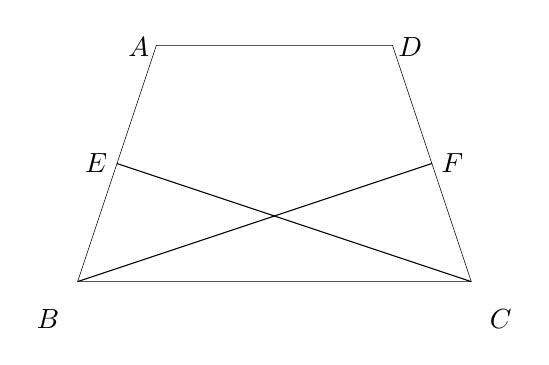
\begin{tikzpicture}
	% 定义多个点(a/b/<name>):坐标(a, b), 名称<name>
	\tkzDefPoints{-2.5/0/B, 2.5/0/C, -1.5/3/A,%
	 1.5/3/D, 0/1.5/O}
	%% 调用Euclide包中的函数进行操作:求中点, 垂线 
	%% 定义一个点-->中间不能加空格(A, B)
	% 会报错得到这个点(设为变量E)
	\tkzDefMidPoint(A,B)   \tkzGetPoint{E}
	\tkzDefMidPoint(C,D)   \tkzGetPoint{F}
	%% 连接点
	\tkzDrawPolygon(A, B, C, D)
	%% 可以使用tikz命令来连接euclide定义的点, 它们二者兼容
	\draw (B) -- (F)node[right]{$F$};
	\draw (C) -- (E)node[left]{$E$};
	%% 以O为中心自动填充标签ABCD。不用加$$
	\tkzAutoLabelPoints[center=O](A,B,C,D) 
\end{tikzpicture}
\end{example}

%\vspace*{5em}
\begin{example}
	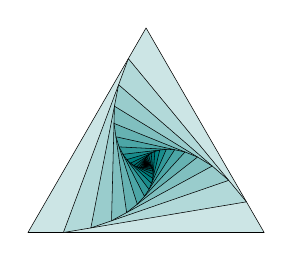
\begin{tikzpicture}[scale=.25]
		\tkzDefPoints{00/0/A,12/0/B,6/12*sind(60)/C}
		\foreach \density in {20,30,...,240}{%
		\tkzDrawPolygon[fill=teal!\density](A,B,C)
		\pgfnodealias{X}{A}
		\tkzDefPointWith[linear,K=.15](A,B) \tkzGetPoint{A}
		\tkzDefPointWith[linear,K=.15](B,C) \tkzGetPoint{B}
		\tkzDefPointWith[linear,K=.15](C,X) \tkzGetPoint{C}}
	\end{tikzpicture}    
\end{example}

\begin{example}
	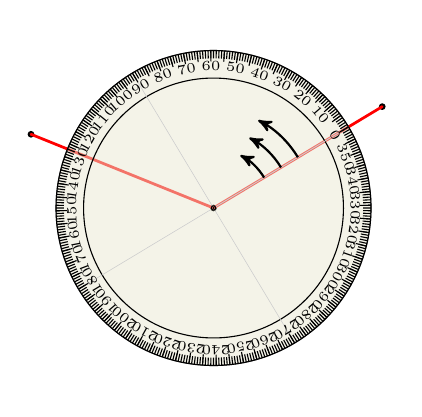
\begin{tikzpicture}[scale=.5]
		\tkzDefPoint(2,0){A}\tkzDefPoint(0,0){O}
		\tkzDefShiftPoint[A](31:5){B}
		\tkzDefShiftPoint[A](158:5){C}
		\tkzDrawPoints(A,B,C)
		\tkzDrawSegments[color = red,
		line width = 1pt](A,B A,C)
		\tkzProtractor[scale = 1](A,B)
	\end{tikzpicture}
\end{example}

\begin{example}
	\begin{tikzpicture}[scale=.75,rotate=-30]
		\tkzDefPoint(0,0){O}
		\tkzDefPoint(4,-5){A}
		\tkzDefIntSimilitudeCenter(O,3)(A,1)
		\tkzGetPoint{I}
		\tkzExtSimilitudeCenter(O,3)(A,1)
		\tkzGetPoint{J}
		\tkzDefTangent[from with R= I](O,3 cm)
		\tkzGetPoints{D}{E}
		\tkzDefTangent[from with R= I](A,1 cm)
		\tkzGetPoints{D'}{E'}
		\tkzDefTangent[from
		with R= J](O,3 cm)
		\tkzGetPoints{F}{G}
		\tkzDefTangent[from with R= J](A,1 cm)
		\tkzGetPoints{F'}{G'}
		\tkzDrawCircle[R,fill=red!50,opacity=.3](O,3 cm)
		\tkzDrawCircle[R,fill=blue!50,opacity=.3](A,1 cm)
		\tkzDrawSegments[add = .5 and .5,color=red](D,D' E,E')
		\tkzDrawSegments[add= 0 and 0.25,color=blue](J,F J,G)
		\tkzDrawPoints(O,A,I,J,D,E,F,G,D',E',F',G')
		\tkzLabelPoints[font=\scriptsize](O,A,I,J,D,E,F,G,D',E',F',G')
	\end{tikzpicture}
\end{example}


\begin{example}
	\begin{tikzpicture}[scale=.8]
	    \tkzDefPoint(3,3){c}
	    \tkzDefPoint(6,3){a0}
	    \tkzRadius=1 cm
	    \tkzDrawCircle[R](c,\tkzRadius)
	    \foreach \an in {0,10,...,350}{
	    \tkzDefPointBy[rotation=center c angle \an](a0)
	    \tkzGetPoint{a}
	    \tkzDefTangent[from with R = a](c,\tkzRadius)
	    \tkzGetPoints{e}{f}
	    \tkzDrawLines[color=magenta](a,f a,e)
	    \tkzDrawSegments(c,e c,f)
	    }%
	\end{tikzpicture}
\end{example}




\section{TiKZ软件}
\subsection{TiKZ in mathcha}
\tikzset{every picture/.style={line width=0.75pt}} %set default line width to 0.75pt  
 
\begin{center}     
	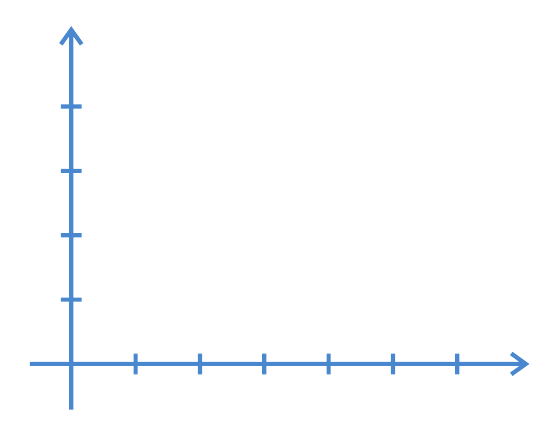
\begin{tikzpicture}[x=0.75pt,y=0.75pt,yscale=-1,xscale=1]
	%uncomment if require: \path (0,235); %set diagram left start at 0, and has height of 235
	%Shape: Axis 2D [id:dp048941842347560494] 
	\draw [color={rgb, 255:red, 73; green, 135; blue, 206},
		  draw opacity=1 
		][line width=1.5] (41,177) -- (280,177)(61,16) -- (61,199) (273,172) -- (280,177) -- (273,182) (56,23) -- %
		(61,16) -- (66,23) (92,172) -- (92,182)(123,172) -- (123,182)(154,172) -- (154,182)(185,172) -- % 
		(185,182)(216,172) -- (216,182)(247,172) -- (247,182)(56,146) -- (66,146)(56,115) -- %
		(66,115)(56,84) -- (66,84)(56,53) -- (66,53);
	\end{tikzpicture}
\end{center}





\end{document}


